%
% File acl2017.tex
%
%% Based on the style files for ACL-2015, with some improvements
%%  taken from the NAACL-2016 style
%% Based on the style files for ACL-2014, which were, in turn,
%% based on ACL-2013, ACL-2012, ACL-2011, ACL-2010, ACL-IJCNLP-2009,
%% EACL-2009, IJCNLP-2008...
%% Based on the style files for EACL 2006 by 
%%e.agirre@ehu.es or Sergi.Balari@uab.es
%% and that of ACL 08 by Joakim Nivre and Noah Smith

\documentclass[11pt,a4paper]{article}
\usepackage{graphicx}
\usepackage[hyperref]{acl2017}
\usepackage{times}
\usepackage{latexsym}

\usepackage{url}

\aclfinalcopy % Uncomment this line for the final submission
%\def\aclpaperid{***} %  Enter the acl Paper ID here

\setlength\titlebox{10cm}
% You can expand the titlebox if you need extra space
% to show all the authors. Please do not make the titlebox
% smaller than 5cm (the original size); we will check this
% in the camera-ready version and ask you to change it back.

\newcommand\BibTeX{B{\sc ib}\TeX}

\title{Hack Harassment: Technology Solutions to Combat Online Harassment}

\author{George W. Kennedy III \\ Intel \\ Hillsboro, OR \\ \tt {george.w.kennedy@intel.com} \And Andrew W. McCollough \\ EdgeRock Technology Partners\\ Hillsboro, OR \\ \AND Edward Dixon \\ Intel \\ Cork, Ireland \\ \tt {edward.dixon@intel.com} \\ \And Alexie Bastidas \\ Intel \\ Santa Clara, CA \\ \And John Ryan \\ Intel \\ Cork, Ireland \And Chris Loo \\ Intel \\ Santa Clara, CA  \And Saurav Sahay \\ Intel \\ Santa Clara, CA }  

\date{}

\begin{document}
\maketitle
\begin{abstract}
  This work is part of a new initiative to use machine
  learning to identify online harassment in social media
  and comment streams. Online harassment goes
  under-reported due to the reliance on humans to
  identify and report harassment, reporting that is further
  slowed by requirements to fill out forms
  providing context. In addition, the time for moderators
  to respond and apply human judgment can
  take days, but response times in terms of minutes
  are needed in the online context. Though some of
  the major social media companies have been doing
  proprietary work in automating the detection of
  harassment, there are few tools available for use by
  the public. In addition, the amount of labeled online
  harassment data and availability of cross platform
  online harassment datasets is limited. We present
  the methodology used to create a harassment dataset
  and classifier and the dataset used to help the
  system learn what harassment looks like.

\end{abstract}

\section{Introduction}

Online harassment has been a problem to a greater
or lesser extent since the early days of the internet.
Previous work has applied anti-spam techniques
like machine learning based text classification 
~\cite{Reynolds:2011} to
detecting harassing messages. However, existing
public datasets are limited in size, with labels of
varying quality.

The \#HackHarassment ~\cite{HH:2017} initiative 
(an alliance of tech companies and
NGOs devoted to fighting bullying on the internet)
has begun to address this issue by creating a web
tool to collect and label data, and using the tool to
generate a large, high-quality, cross-platform dataset.
The release of this tool is scheduled for Summer
2017. As we complete further rounds of labelling
with a public audience, later iterations of this dataset
will increase the available samples by at least
an order of magnitude and enable corresponding
improvements in the quality of machine learning
models we have built for harassment detection. In
this paper, we introduce an improved cross-platform
harassment dataset and a machine learning
model built on the dataset.

\section{Related Work}

Previous work in the area by ~\cite{Bayzick:2011} showed that natural language
processing in combination with a rule-based
system could detect bullying messages on an
online forum, but with very poor accuracy. However,
the same work also made clear that the limiting
factor on such models was the availability of a
suitable quantity of labeled examples, e.g. the
Bayzick work relied on a dataset of 2,696 samples,
only 196 of which were found to be examples of
bullying behavior. Additionally, this work relied
on classical decision-tree models like J48 and
JRIP, and k-nearest neighbors classifiers like IBk,
as opposed to modern ensemble methods or deep
neural-network-based approaches. In addition, Intel's
\#HackHarassment team published work ~\cite{Bastidas:2016} showing results for harassment
detection using a variety of model types on a new
dataset of comments and posts which their team
had labelled.

More recently, major internet companies have
focused efforts on combating various forms of harassment
online. Yahoo researchers have developed
machine learning models for detecting abusive
language ~\cite{Nobata:2016a} and a Google Jigsaw team partnered
with the Wikimedia Foundation to develop
solutions for reducing personal attacks or ‘toxic
comments’, in Wikimedia editing ~\cite{Wulczyn:2017}. Nobata outperformed
state-of-the-art deep learning approaches
with their supervised learning approach
using a combination of linguistic, n-gram (including
character n-grams), syntactic (POS), and semantic
(using comment embeddings similar to
word2vec) features. In addition, the Yahoo team
has released the longitudinal New Feed data set
used in the study on ~\cite{Webscope:2017}. Wulczyn
demonstrated that their machine models can perform
as well as three human graders in identifying
toxic comments in Wikipedia editing wars, and in
addition released the Perspective API to enable developers
to utilize their solution. However, see
~\cite{Hosseini:2017}
for comments on adversarial attacks and the resultant
fragility of the model - and other models that
depend on token-level features. We extend these
results and others by developing a system architecture
for crowdsourcing sample labeling, a crosssocial-media-platform
dataset, and providing an
open source classifier for developers to build upon.
The classifier is intended to be open sourced in
Summer 2017.

\section{Methods}

In this work, we build upon our initial results using
version 1.0 of our dataset ~\cite{Bastidas:2016}. We followed a supervised classification
method that uses a data with gold-standard labeled
comments and a set discriminating linguistic properties,
or features, of each comment to predict the
class membership of new or untrained comments.
Our features consisted primarily of n-gram
and a small set of linguistic features on datasets
drawn from The Guardian, Reddit, and Twitter. We
performed no significant pre-processing on the
data other than tokenization, though in the future
we anticipate adding further feature-reduction
steps, such as stemming, to improve model performance.

\section{Data Source Selection}

Three initial data sources were selected: The
Guardian, Reddit, and Twitter. Text from each data
source were extracted in several ways in Summer
2016. Comments on polarizing or hot-button news
articles were extracted from the Guardian, an
online news source. Comments from Reddit, a
popular social media site, were selected from comment
which had received at least 100 down votes.
Short texts from Twitter, “tweets” were hand-curated
from an initially machine-selected data set
from Twitter, and then further tweets scraped by
searching on polarizing or hot-button topics.

\subsection{Reddit}
Comments from Reddit were downloaded from a
publicly available dataset on Google BigQuery,
reddit\_comments\_all\_2015. These comments
were then filtered to those that had received at least
100 down votes. We used our initial version of the
classifier to label these comments. The resulting
5700 harassing comments were then further manually
labeled by an in-house team of analysts. Analysts
were given instructions and examples for
annotation of harassment or non-harassment. In
addition, the raters were provided with an additional
set of more fine-grained labels but instruction
on annotation was not provided.). Each post
was labeled independently by at least five Intel Security
Web Analysts. A perfect consensus was relatively
rare, and so we rated a post as “harassing”
if 40\%, 2 of our 5 raters, consider it to be harassing.

\subsection{Twitter}
Data were comprised of two sources: manual curation
and annotation of a pre-existing machine-annotated
dataset and a set of scraped tweets using
proprietary sampling methods. The sampling
should not be considered unbiased. The initial
$~5000$ tweets were sourced from an online repository
of tweets at. Additional tweets were scraped
directly from Twitter during July 2016 using a custom
twitterbot that queried on hot-button topics as
keywords to the Twitter API. These additional
tweets were first labeled by our early classifier and
then manually labeled by our team ~\cite{Hart:2016}.

\subsection{The Guardian}
Comments were scraped from 15 articles covering
hot-button or polarizing topics. We believe that
minimal harassing comments were found in the
Guardian dataset as Guardian comments are curated
by a team of moderators in accordance with
their content policy. Therefore, minimal or no harassing
comments should be expected, as we confirmed
in the dataset.

\begin{figure}
  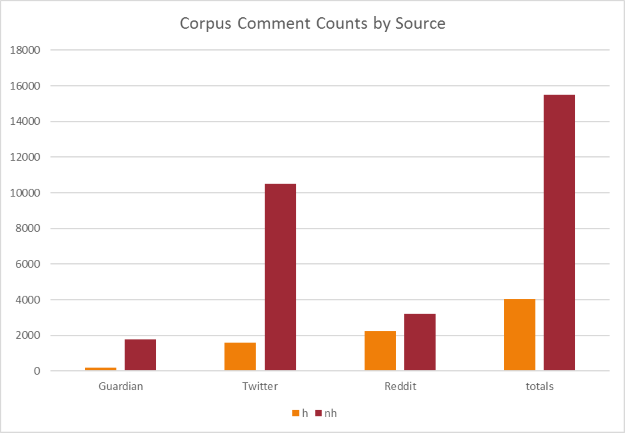
\includegraphics[width=\linewidth]{figure1_corpus_counts_by_source.png}
  \caption{Corpus Comment Counts by Source}
  \label{fig:corpus}
\end{figure}


Figure \ref{fig:corpus} shows that the current data set is reasonably unbalanced overall with a $~1:4$ ratio of non-harassing to harassing comments. In addition, the categories are unbalanced across source as well as category within source, such that Reddit, despite being only 28\% of the total comments contributed 56\% of the harassing comments.

\begin{figure}
  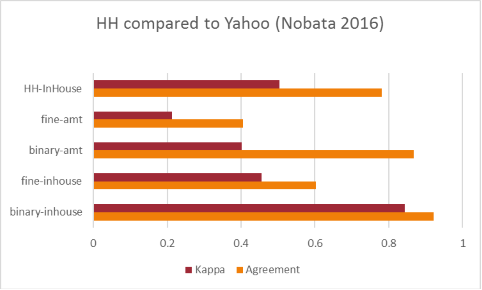
\includegraphics[width=\linewidth]{figure2_iaa.png}
  \caption{Inter-annotator agreement for Hack Harassment (HH) compared to Yahoo. HH uses Krippendorf’s Alpha and Yahoo uses Kappa. Agreement is an average pairwise agreement.}
  \label{fig:iaa}
\end{figure}

\begin{figure}
  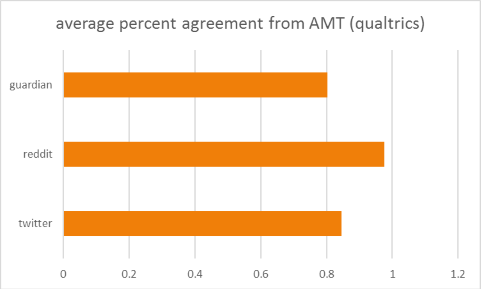
\includegraphics[width=\linewidth]{figure3_average_percent_agreement_amt.png}
  \caption{Average Percent of Agreement Among Amazon Mechanical Turk (AMT) Annotators}
  \label{fig:amt}
\end{figure}

As shown in Figure \ref{fig:iaa} and Figure \ref{fig:amt}, average agreement
is below 90\% for the Guardian and Twitter
surveys, with an average across all Qualtrics surveys
only .875. This is well below what is typically
suggested for raw agreement scores.

\begin{table}[h]
\begin{center}
\begin{tabular}{|l|rl|}
\hline \bf Guardian URLs \\ \hline
https://www.theguardian.com/discussion/p/4pcq2 \\
https://www.theguardian.com/discussion/p/4pgek \\
https://www.theguardian.com/discussion/p/4an9q \\
https://www.theguardian.com/discussion/p/4p76x \\
https://www.theguardian.com/discussion/p/4pdqd \\
https://www.theguardian.com/discussion/p/4phck \\
https://www.theguardian.com/discussion/p/4pf70 \\
https://www.theguardian.com/discussion/p/4pfe3 \\
https://www.theguardian.com/discussion/p/4k4tx \\
https://www.theguardian.com/discussion/p/4pd76 \\
https://www.theguardian.com/discussion/p/4jmg2 \\
https://www.theguardian.com/discussion/p/4pg57 \\
https://www.theguardian.com/discussion/p/4p6dt \\
https://www.theguardian.com/discussion/p/4p6gn \\
https://www.theguardian.com/discussion/p/4pgbx \\
\hline
\end{tabular}
\end{center}
\caption{\label{font-table} Guardian URLs used to scrape initial comments. }
\end{table}

\section{Data Ingest and Annotation Methods}
Data ingest process and annotation were heterogeneous
in nature. Manual curation was combined
with machine annotation in several iterated steps to
produce a final annotated dataset. The comment dataset
was simply annotated with a Boolean indicating
harassment. Harassment was determined on the
gold data through a percent voting method: the reported
metrics are for 40\% and above simple agreement
among raters that a given comment is harassment.

All preprocessing, training and evaluation was
carried out in Python, using the popular SciKitLearn
(for feature engineering and linear models)
in combination with Numpy3 (for matrix operations)
~\cite{Pedregosa:2011,van_der_Walt:2011}.

\section{Feature Selection}
Features were generated by tokenizing each comment,
hashing the resulting n-grams, and computing
a TF/IDF value for each token. The resultant
feature vectors were used to train a Random Forest
classifier. We used the following features:

\begin{itemize}
\item Unigram and Bigram TF-IDF: this is a
standard feature used in text-categorization.
We used unigrams and bigrams. Trigrams
were not used because the size of the dataset
meant almost all trigrams were too rare for
their presence and absence to reach statistical
significance.
\item Character N-Gram TF-IDF from 3 to 6
characters: The goal with this was to target
common alternative spellings of words, particularly
frequent in online communication.
\item Unigram Token Count: we utilized
NLTK’s Twitter Tokenizer to tokenize the
tokens and count the number of tokens. The
Twitter Tokenizer handles URLs and
Hashtags much better than a standard
punctuation based tokenizers found in NLTK
or Sck-kit Learn. Our assumption behind
using token count is that harassing texts tend
to be brief assaults rather than long diatribes.
\item Source: In combination with the token
count, we selected a dummy coefficient (toggled
as 1 or 0) to highlight if a comment is
sourced from Twitter or not.
\item Sentiment Polarities: we utilized NLTK’s
VADER Sentiment Analyzer to generate sentiment
polarities for positive, neutral, and
negative sentiment. Our assumption was that
harassing comments tend to have more negative
sentiment, whereas non-harassing comments
tend to have more positive sentiment.
\end{itemize}

\section{Training Dataset}
The current training dataset contains: 20,432
unique comments. Of these comments, 4136 are labeled
as harassment, 16296 are labeled as non-harassment.
12,049 comments are sourced from Twitter,
with the remaining 8383 being from Reddit or
the Guardian.

\section{Machine Learning Model}
Bastidas tested a variety of algorithms, including
SVM, Decision Tree, Random Forest (ensemble
Decision Trees), and Multinomial Naïve Bayes
\cite{Bastidas:2016}. We increased the size of the
Reddit dataset and included labeled comments that
were sampled from Twitter and The Guardian. We
collected performance results using this larger,
cross-platform dataset, described in the Data
Source Selection section, and a Scikit-Learn Random
Forest classifier. For our hyperparameters we
limited the number of trees to 200 and left the tree
depth unbounded. Subsequently, the data were
trained on the Random Forest by splitting the dataset
into 80/20 training and evaluation sets, and
then the training data were further split into Kfold
(n=10) folds for cross-validation and the average
results reported in Table 2. Of primary concern to
us is to optimize for high recall. We want to minimize
our false-negative rate for harassment.

\begin{table}[h]
\begin{center}
\begin{tabular}{|l|l|l|l|}
\hline \bf Class & \bf Precision & \bf Recall & \bf F1 Score \\ \hline
Not Harassing & 0.93 & 0.95 & 0.94 \\
Harassing & 0.75 & 0.68 & 0.71 \\
Average & 0.89 & 0.90 & 0.90 \\
\hline
\end{tabular}
\end{center}
\caption{Random forest classifier results. }
\end{table}

\section{Future Work}
New work from Facebook and OpenAI on text
classification suggests obvious next steps. Bytelevel
deep neural nets are capable of state-of-theart
results on large datasets, can exploit unlabeled
data, as described in recent work from OpenAI
~\cite{Radford:2017} and
have the potential to resist the "adversarial" tokens
described in ~\cite{Hosseini:2017}. Using OpenAI's approach with a large,
unlabeled dataset for pre-training is an obvious
next step. A contrasting approach that requires further
evaluation is the FastText model from Facebook's
Advanced Research Lab, which, as described
in ~\cite{Joulin:2016} and ~\cite{Bojanowski:2016}, is competitive with deep convolutional
neural networks and can exploit unlabeled
data using pre-trained WordVectors, while requiring
vastly less training time than competitive
alternatives.

\section{Conclusion}
We have presented to our cross-platform harassment
dataset, machine learning model. We intend
to open our labeling platform to the public to expand
the Hack Harassment cross platform dataset.
As we complete further rounds of labelling with a
public audience, later iterations of this dataset will
increase the available samples by at least an order
of magnitude, enabling corresponding improvements
in the quality of machine learning models
for harassment detection. We look forward to both
the availability of a larger, cross-social-mediaplatform
harassment dataset and seeing the development
of classifiers that improve upon our work.
We welcome partners able to contribute to expanding
the dataset and improving the modeling.




% include your own bib file like this:
%\bibliographystyle{acl}
%\bibliography{acl2017}
\bibliography{acl2017}
\bibliographystyle{acl_natbib}

\end{document}
